

\section{Problem Instance}
This project and report will focus and analyse instances with a single divisible good, which will be denoted as $\sTheCake$, this simplification does not reduce the generality of having multiple cakes on its own, as a set of cakes can be combined into a single divisible heterogenous cake. this project however focuses on instances with homogenous cake(s), so this generalization is not applicable as agents can value cakes differently, meaning combining multiple homogenous cakes would also result in a heterogenous cake.

In short, instances, $\sInstance$, considered in this project consists of the following:
\begin{itemize}
    \item set of agents: $\sAgent\in\sAllAgents=\{1,2,...,\sNumAgents\}$.
    \item set of indivisible items: $\sItem\in\sAllItems=\{1,2,...,\sNumItems\}$
    \item single divisible good (cake): $\sTheCake$, where a piece of cake of size $z$ is $\sTheCake_z=\sTheCake_{[0,z]}$.
    \item set of goods: $\sGood\in\sAllGoods=\{1,2,...,\sNumGoods\}:=\sAllItems\cup\sTheCake$.
    \item set of valuation functions $\sValuation \in \sAllValuations$ where $\sValuation_\sAgent$ is the valuation function for agent $\sAgent$.
\end{itemize}



\subsection{Cake Sizes}\label{subsec:cake-sizes}
In order to compare the algorithms for different types of cakes later the instances are split into four main categories. 

\subsubsection*{Small Cake}\label{subsubsec:small-cake}
A Cake is considered \textit{small} if the value of the entire cake for each agent is equal to or less than the value of any indivisible item See \autoref{fig:visualize_instance_small_cake} for example. Formally:
$$\forall\sAgent\in\sAllAgents, \forall\sItem\in\sAllItems, \sValuation_\sAgent(\sTheCake)\leq \sValuation_\sAgent(\sItem)$$
\begin{figure}
    \centering
    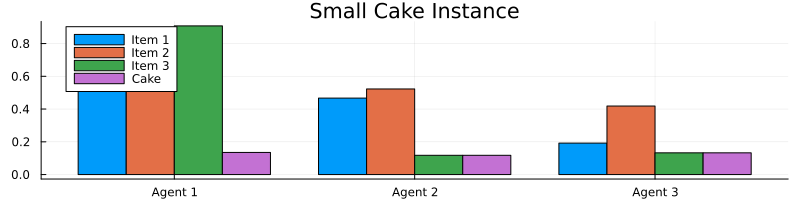
\includegraphics[width=\textwidth]{instance_small.png}
    \caption{Visualization of agents valuations for an instance with a \textit{small cake}.}
    \label{fig:visualize_instance_small_cake}
\end{figure}

\subsubsection*{Medium Cake}\label{subsubsec:medium-cake}
A Cake is considered \textit{medium} if the value of the entire cake for each agent is larger than, or equal to the smallest item, and smaller than or equal to the agents largest item. See \autoref{fig:visualize_instance_medium_cake} for an example. Formally:
$$\forall\sAgent\in\sAllAgents, \exists\sItem_1,\sItem_2\in\sAllItems, \sValuation_\sAgent(\sItem_1)\leq\sValuation_\sAgent(\sTheCake)\leq\sValuation_\sAgent(\sItem_2)$$
\begin{figure}
    \centering
    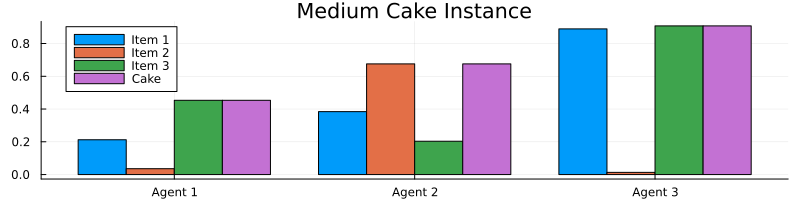
\includegraphics[width=\textwidth]{instance_medium.png}
    \caption{Visualization of agents valuations for an instance with a \textit{medium cake}.}
    \label{fig:visualize_instance_medium_cake}
\end{figure}

\subsubsection*{Large Cake}\label{subsubsec:large-cake}
A Cake is considered \textit{large} if the value of the entire cake for each agent is equal to or larger than the sum of the value of all indivisible items. Formally: 
$$\forall\sAgent\in\sAllAgents, \sValuation_\sAgent(\sTheCake)\geq \sum_{\sItem\in\sAllItems}\sValuation_\sAgent(\sItem)$$
\begin{figure}
    \centering
    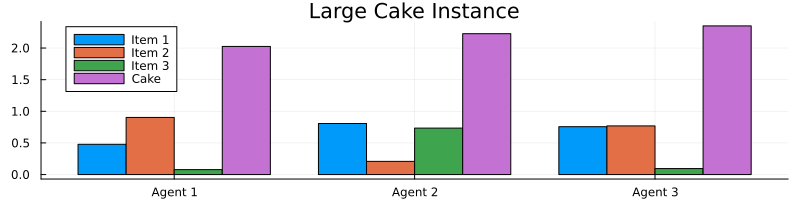
\includegraphics[width=\textwidth]{instance_large.png}
    \caption{Visualization of agents valuations for an instance with a \textit{large cake}.}
    \label{fig:visualize_instance_large_cake}
\end{figure}

\subsubsection{Individual Cake}\label{subsubsec:individual-cake}
Finally we have instances with individual cake, meaning that each agent are free to value the cake however they want compared to their indivisible items. In other words, in these instances one agent could value the cake as a \textit{large} cake, while another agent sees it as a \textit{small} cake, hence the name "individual".
\begin{figure}
    \centering
    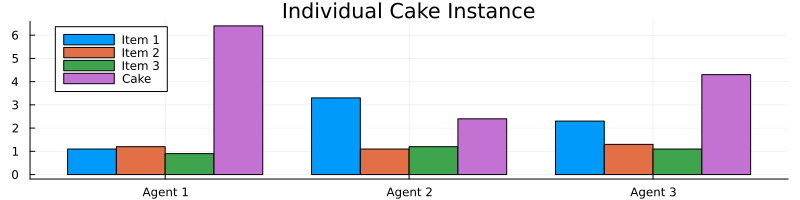
\includegraphics[width=\textwidth]{instance_individual.png}
    \caption{Visualization of agents valuations for an instance with a \textit{variable cake}.}
    \label{fig:visualize_instance_variable_cake}
\end{figure}

Together these four categories of cake covers all possible mixed instances with a single divisible good, and lets us easier examine and compare results for different types of cakes in \autoref{chp:results} and \autoref{sec:discussion}.